\documentclass[a4paper,14pt, twocolumn]{extarticle}
\usepackage{geometry} % Bigger font size for article

% make it more readable non-serif
\usepackage{lmodern}
\usepackage[T1]{fontenc} % i.a. makes title font non-serif
\renewcommand{\familydefault}{\sfdefault}
\usepackage{titlesec}

%monospace font command for codes
\usepackage{alltt}
\def\code#1{
	\begin{alltt}
	\texttt{#1}
	\end{alltt}
}

%remove newline after subsubsection sections
\usepackage{titlesec}
\titleformat{\subsubsection}[runin]{\normalfont\normalsize\bfseries}{\thesubsubsection}{1em}{}

% reduce numbering
\setcounter{secnumdepth}{2}

% hungarian language
\PassOptionsToPackage{defaults=hu-min,classmod=unchanged}{magyar.ldf}
\usepackage{t1enc}
\usepackage[magyar]{babel}
\selectlanguage{magyar}
\usepackage[utf8]{inputenc}

% compacitem
\usepackage{paralist}


% images 
\usepackage{graphicx}
\graphicspath{ {./images/} }

% set smaller margins
\addtolength{\oddsidemargin}{-1.2cm}
\addtolength{\evensidemargin}{-1.2cm}
\addtolength{\textwidth}{2.4cm}
\addtolength{\topmargin}{-1.5cm}
\addtolength{\textheight}{3cm}

% remove red color for hyperref in TOC (maybe only in Adobe reader)
\usepackage[unicode]{hyperref}
\hypersetup{
	colorlinks,
	citecolor=black,
	filecolor=black,
	linkcolor=black,
	urlcolor=black
}



\begin{document}
	\onecolumn
	
	\begin{titlepage}
	\begin{center}
		{\LARGE\textbf{Tesztautomatizálás alapjai}}
	\end{center}
	\vfill
	\begin{center}
		{\large Utoljára módosítva: \today}
		\vspace{0.5cm}
		
		{Készítette: Ráncsik Áron}
	\end{center}
\end{titlepage}	
	\tableofcontents
	
	\twocolumn
	
	\leavevmode\thispagestyle{empty}\newpage
	\leavevmode\thispagestyle{empty}\newpage
	\section{TTCN}
	\section{Tesztelés minőségbiztosítás és adatbiztonság szempontból}
		\subsection{Fogalmak}
			\subsubsection{Etikus hacker}
				\begin{compactitem}
					\item A vizsgálandó cég által megbízva 
					\item Aláírt szerződés, engedély, titoktartási nyilatkozat és károk alól felmentés 
					\item Az előzetes engedély nélküli hibakeresés és a hiba kihasználása Magyarországon bűncselekmény (de legalábbis szürke zóna) 
					\item Vannak azonban “jó fej” cégek akik díjazzák a hibabejelentést, és “bounty” programokat működtetnek. 
					\item Alapvetően nem szabad erre számítani. 
				\end{compactitem}
			\subsubsection{Kockázat}
			\begin{compactitem}
				\item Hatás (veszteség)
				\item Valószínűség
				\item Védekezés
				{ 
					\begin{compactitem}
						\item Költség
					\end{compactitem}
				}
				\item Támadó
				{ 
					\begin{compactitem}
						\item Költség
						\item Kockázat
						\item Nyereség
					\end{compactitem}
				}
			\end{compactitem}
			\newpage
			\subsubsection{Kockázatelemzés egy módszere a támadás-fa elemzés} 
				\begin{compactitem}
					\item A  támadó szempontjából közelíted meg magad
					\begin{center}
						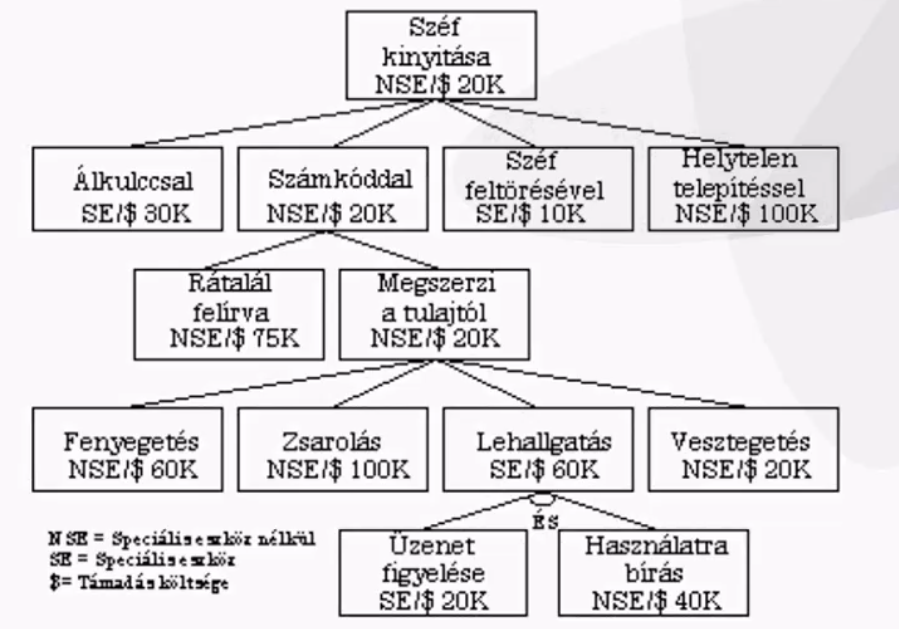
\includegraphics[width=10cm]{tamadasfa}
					\end{center}
				\end{compactitem}
			\subsubsection{Vagyon}
				\begin{compactitem}
					\item Adatok
					{ 
						\begin{compactitem}
							\item Ügyféladatok
							\item Üzleti titkok 
							\item Forráskód
							\item Dokumentáció
							\item e-mailek
							\item Alkalmazottak adatai
						\end{compactitem}
					}
					\item Eszköz: prototípus
					\item Egyéb: hírnév bizalom
				\end{compactitem}		
			\subsubsection{Vagyon értéke}
				\begin{compactitem}
					\item Jövőbeni jövedelem 
					\item Érték a konkurenciának 
					\item Újragyártás költsége 
					\item Büntetés a vagyon hiánya miatt (pl. adóellenőrzés) 
					\item Helyreállítási költség adatvesztés miatt 
					\item Büntetés adatvesztés miatt 
					\item Cég értékének csökkenése 
				\end{compactitem}
		\subsection{Adatokhoz való hozzáférés és biztonság}
			\begin{compactitem}
				\item Hozzáférés
				{
					\begin{compactitem}
					\item Helyi hálózat 
					\item VPN 
					\item Fizikai (CD, Pendrive) 
					\item Email 
					\end{compactitem}
				}
				\item Biztonság
				{
					\begin{compactitem}
						\item Titkosítás (milyen erősség, ki ismeri a kulcsokat) 
						\item Azonosítás (jelszó, hw kulcs, kettős autentikáció) 
						\item Jogosultságok
					\end{compactitem}
				}
			\end{compactitem}
		\subsection{Kockázatok}
		\begin{compactitem}
			\item Vezetőség támogatásának hiánya 
			\item Források hiánya
			{
				\begin{compactitem}
					\item Tudás hiánya 
					\item Eszközök hiánya 
				\end{compactitem}
			}
			\item Szervezet támogatásának hiánya 
			\item Kulcsemberek támogatásának hiánya 
			\item Biztonsági kockázatok lebecsülése 
			\item A biztonsági tesztelés és a tesztelési előírások eltérése 
			\item A rendszer működésének nem ismerete 
			\item A rendszer céljának nem ismerete
		\end{compactitem}
		\subsection{A biztonsági tesztelés szerepe a software életciklusban}
			Lépései:
			\begin{compactitem}
				\item Követelményfelmérés 
				\item Tervezés 
				\item Fejlesztés 
				\item Tesztelés 
				\item Üzemeltetés 
				\item Dokumentáció
			\end{compactitem}
			\newpage
			
			\subsection{Tesztelés követelményfelmérése}
				\subsubsection{Adatvédelmi igények}
				\begin{compactitem}
					\item felhasználói csoportokat és azok adatvédelmi igényeit azonosítani és dokumentálni \item adattípusokat azononosítani és a biztonsági szinteket hozzárendelni 
					\item felhasználók hozzáférését meghatározni
				\end{compactitem}
			\subsubsection{Biztonsági követelményeknek való megfelelés}
				\begin{compactitem}
					\item Biztonsági követelményeket dokumentálni 
					\item Kivételeket felkutatni
				\end{compactitem}
			\subsubsection{Gyakori sérülékenységek}
				\begin{compactitem}
					\item Az ismert sérülékenységeket dokumentálni és figyelembe venni 
					\item Ismeretlen sérülékenységekre felkészülni
				\end{compactitem}
			\subsubsection{Tesztelhetőség}
				\begin{compactitem}
					\item A követelmények úgy lettek megfogalmazva, hogy az alapján megírhatóak a tesztek? 
					\item Az általános kifejezések (pl. biztonságos adatátvitel vagy hozzáférés csak megfelelő jogokkal) megfelelően definiálva vannak és tesztelhetőek?
				\end{compactitem}
			\subsubsection{Használhatóság}	
				\begin{compactitem}
					\item Egyensúly a használhatóság és a biztonság között 
					\item A követelmények megfelelően szabályozzák a használhatósághoz tartozó biztonsági szabályokat? 
					\item A biztonsági előírások világosak és érthetőek? 
					\item A felhasználó hozzáférési nehézsége esetén követendő eljárások definiálva és dokumentálva vannak?
				\end{compactitem}
			\subsubsection{Teljesítmény}
				\begin{compactitem}
					\item Egyensúly a teljesítmény és a biztonság között 
					\item A követelmények megfelelően szabályozzák a teljesítményhez tartozó biztonsági szabályokat?
				\end{compactitem}
				\newpage 
				
		\subsection{Tesztelés tervezése}
		\begin{compactitem}
			\item Adj vagy kapj bizalmat, de soha ne feltételezz  
			\item Használj biztonságos autentikációt 
			\item Autentikálás után vizsgáld a hozzáférési jogokat 
			\item Tartsd külön az adatokat és az utasításokat (sql injection, buffer overflow) 
			\item Ne hajts végre megbízhatatlan forrásból származó utasítást 
			\item Validáld az adatokat 
			\item Használd helyesen a titkosítást 
			\item Figyelj oda a kényes adatokra 
			\item Legyél tisztában a külső komponensek sebezhetőségeivel 
			\item Mindig vedd figyelembe a felhasználóidat
			\item Funkcionális biztonsági ellenőrzések(pl. pénztáros nem adhat ki egy határnál nagyobb összeget csak a főpénztáros engedélyével)
			{
				\begin{compactitem}
					\item Jelszavak kezelése(pl. nem szöveges formában vannak tárolva) 
					\item Jelszavak feltörés ellen védettek(pl. nem lehet korlátlanul próbálkozni)
				\end{compactitem}
			}
			\item Szerkezeti hozzáférés ellenőrzés
				{
				\begin{compactitem}
					\item felhasználói jogok 
					\item titkosítás
					\item autentikáció
				\end{compactitem}
			}
			\item Biztonságos kódolási szokások
			{
				\begin{compactitem}
					\item HTTP GET kérések nem tartalmazhatnak érzékeny adatokat 
					\item Alkalmazás hibákat az alkalmazás kell hogy lekezelje 
					\item Adatvalidáció és a hibák logolása (SQL injection) 
					\item Adatok ideiglenes tárolása is csak biztonságos formában és csak a szükséges ideig 
					\item Szervizek futtatása csak a minimálisan szükséges jogokkal és sohasem root-ként 
					\item API-k használata direk OS hívások helyett 
					\item Adatok útközbeni titkosítása 
					\item Jövőbiztosság (könnyű tesztelni és karbantartani) 
				\end{compactitem}
			}
			\item Hozzáférés az operációs rendszerhez
				\subitem Ha egy támadó behatolt akkor semmiben sem lehet bízni 
			\item Nyelv sebezhetőségek
				\subitem forráskód fertőzés
				\subitem fordító hiba
			\item OS sebezhetőségek 
			\item Külső fenyegetések
				\subitem DoS
			\item Belső fenyegetések
				\subitem Outsourcing 
				\subitem Elégedetlen alkalmazott 
			\item A tesztelő rendszer sebezhetőségei
		\end{compactitem}
		\subsection{Tesztek fejlesztése}
			\begin{compactitem}
				\item Buffer overflow 
				\item Adatvalidálás 
				\item Fejlesztő által beépített nem kívánatos kód 
				\item Backdoor 
				\begin{compactitem}
					\item tesztelési célból
					\item támadási célból
					\item felsőbb utasításra
				\end{compactitem}
			\end{compactitem}
		
		\subsection{Komponens fejlesztés tesztelése}
			\begin{compactitem}
				\item Egységként kezeld (kívül minden veszélyforrás) 
				\item Bemenő adatok validálása 
				\item Fordító figyelmeztetéseket nem szabad figyelmen kívül hagyni 
				\item Kövesd a biztonsági előírásokat 
				\item Ne bonyolítsd túl 
				\item Alapállapot a tiltás, csak szükség esetén adj engedélyt 
				\item A lehető legkevesebb jogot adj 
				\item Csak a feltétlen szükséges adatokat küld tovább 
				\item A minőségbiztosításnak van értelme 
				\item Code review
			\end{compactitem}
		\subsection{Integráció tesztelése}
			\begin{compactitem}
				\item Az integráció során új hibalehetőségek és biztonsági rések keletkezhetnek 
				\item Ugyanakkor a komponensekben megmaradt biztonsági rések el is tömődhetnek hogy aztán késöbb orvul hátbatámadják a figyelemetlen fejlesztőt 
				\item Smoke testing (olyan teszt gyűjtemény ami jól lefut a rendszeren és módosítás esetén nézzük hogy elfüstöl-e?)
			\end{compactitem}
		\subsection{Rendszer- és elfogadási teszt}
			\begin{compactitem}
				\item Az átvételi feltételeket még a tervezési fázisban kell definiálni 
				\item Az átvételi teszt valós üzemi feltételek között történik 
				\item Helyes és helytelen adatokat és felhasználói viselkedést, ill. a rendszer azokra adott válaszát is szükséges tesztelni 
				\item Tervezett tesztek meglétének ellenőrzése és futtatása, valamint az eredmények értelmezése
			\end{compactitem}
		\subsection{Üzemeltetés ellenőrzése}
			\begin{compactitem}
				\item Rendszeres penetrációs tesztelés 
				\item “Bounty program” 
				\item Definiált és dokumentált hibakezelési eljárások 
				\item Kárminimalizálás és kommunikáció 
				\item Rendszeres adatmentés
			\end{compactitem}
		\subsection{Minőségbiztosítás, Minőségellenőrzés}
			\subsubsection{Minőségbiztosítás}
				Azok az eljárások amik megpróbálják megakadályozni hogy hibát építsünk be 
				\begin{compactitem}
					\item fontos része a kompetencia fejlesztés is: Ki, mit, miért? Mire kell figyelni? (code review, milyen változónevek, mit, hol valósítunk meg, milyen dokumentáció, visszakövethetőség) 
				\end{compactitem}
			\subsubsection{Minőségellenőrzés}
				tesztek futtatása hogy észrevegyük a beépített hibákat mielött az ügyfél teszi azt.

		\onecolumn
			\subsection{Product quality}
			\begin{center}
				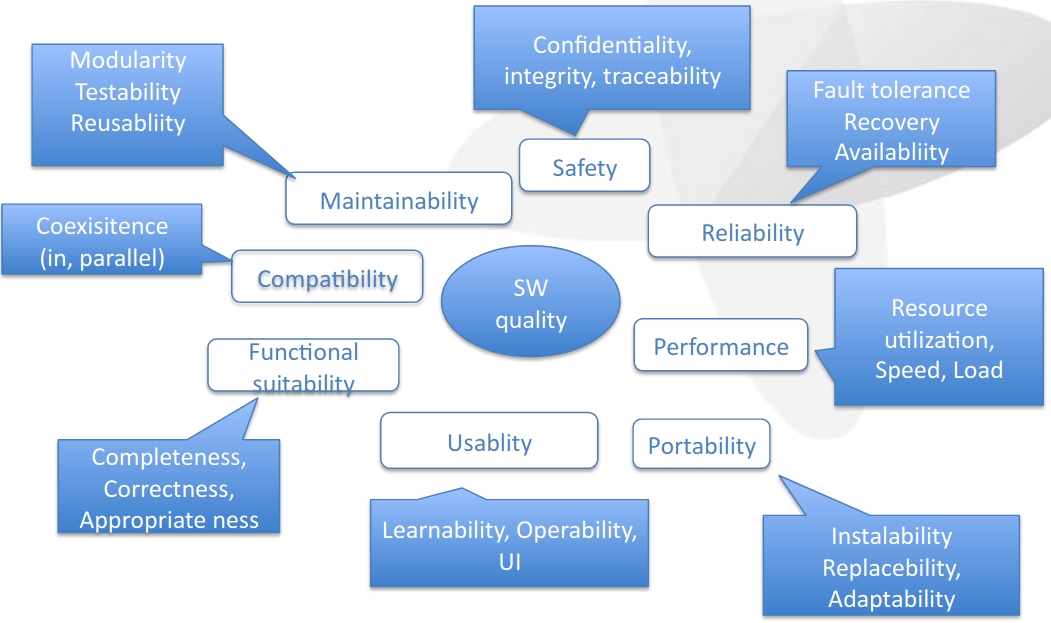
\includegraphics[width=18cm]{pq}
			\end{center}
		\twocolumn
		
		
	\section{Continuous Integration}
		\subsection{What’s in for the developer?}
			\begin{center}
				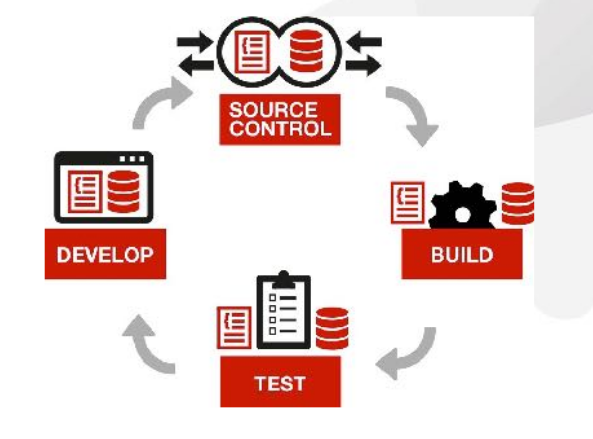
\includegraphics[width=7cm]{ci1}
			\end{center}
		\subsection{Fogalmak}
			\subsubsection{Continuous integration}
				The practice of automatically building and unit testing an entire application frequently, ideally on every source code check-in
				\begin{compactitem}
					\item frequent check-ins 
					\item no long-running parallel code branches 
					\item build and test locally before submitting 
					\item shortening the feedback loop for every change
				\end{compactitem}
		\subsubsection{Continuous delivery}
			The practice of deploying every build to a production-like environment and performing automated integration and acceptance testing 
			\begin{compactitem}
				\item small-scale deployment on a single server 
				\item mock environments with Docker containers or VM 
				\item mimic production environment 
				\item should end with deployment to a production-like environment 
				\item to see functionality and performance in a real environment
			\end{compactitem}
		\subsubsection{Continuous deployment}
			The practice of automatically deploying every build to production after it passes its automated tests
				\begin{compactitem}
					\item every change goes through full automated testing 
					\item deployed automatically to the production environment 
					\item one small change at a time! 
					\item no giant releases with hundreds of changes piled up for months
				\end{compactitem}
		\onecolumn
		\subsection{Összehasonlítás}
		\begin{center}
			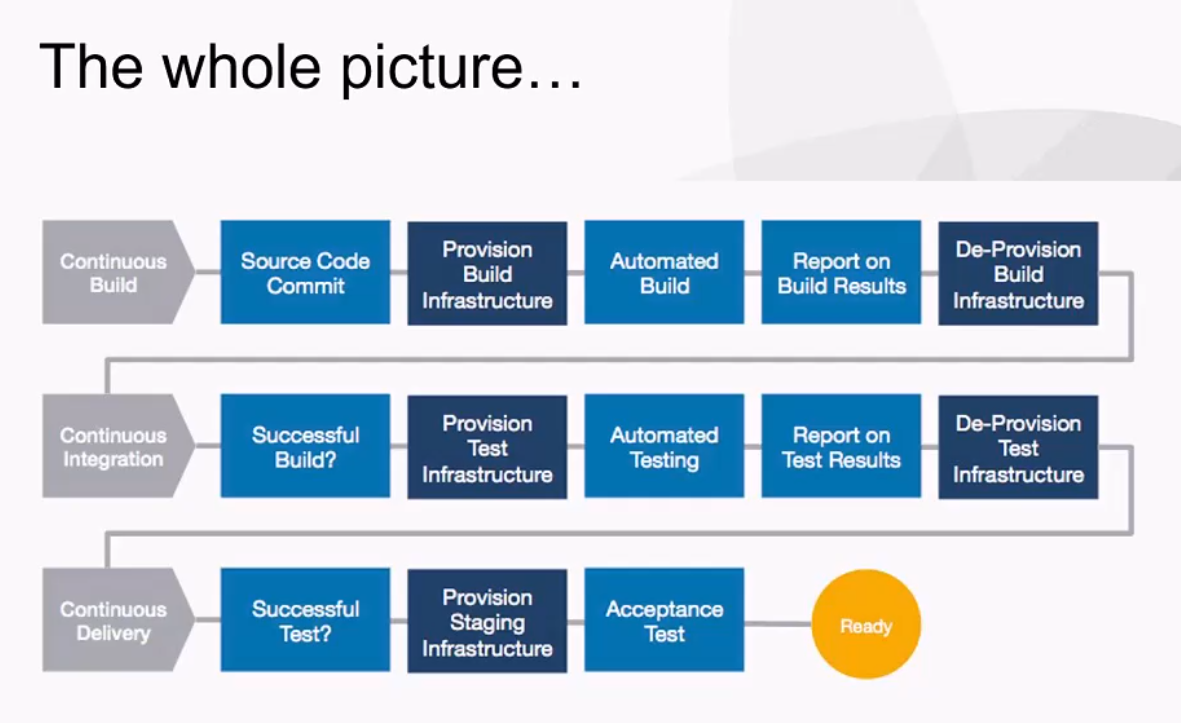
\includegraphics[width=16cm]{ciWhole}
		\end{center}
		\begin{center}
			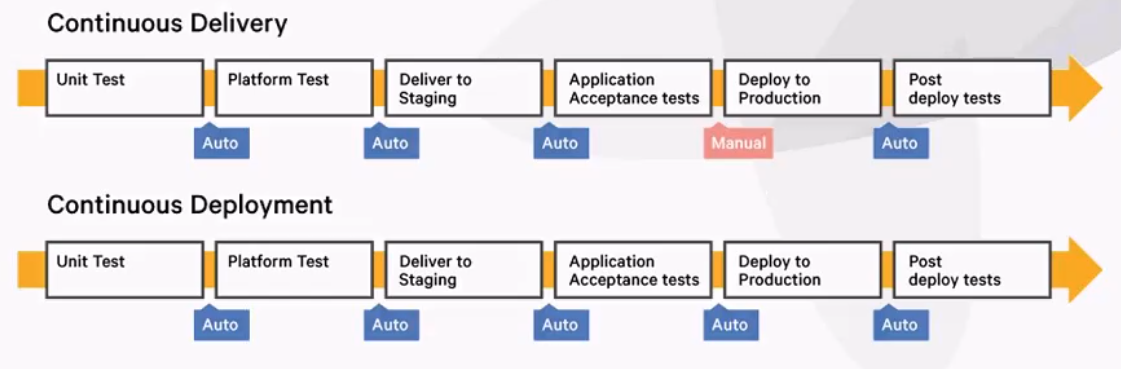
\includegraphics[width=16cm]{cdcd}
		\end{center}
		\newpage
		\subsection{Benefits CI, CDip}
		\begin{compactitem}
			\item empowering teams
			\begin{compactitem}
				\item self service system 
				\item transparent and understandable process of delivery 
				\item makes the team less reactive 
				\item reduces the strain between
				\begin{compactitem}
					\item developers and operation 
					\item QA and security
				\end{compactitem}
			\end{compactitem}
			\item Lowered cycle times
			\begin{compactitem}
				\item from weeks or months to hours or even minutes
			\end{compactitem}
			\item Better security
			\begin{compactitem}
				\item less time remediating security issues 
				\item easier compliance audits
			\end{compactitem}
			\item Rhythm of practice
			\begin{compactitem}
				\item removes stress 
				\item release date is not a stressful event any more
			\end{compactitem}
			\item More time to be productive
			\begin{compactitem}
				\item less time reworking, more time adding new features
			\end{compactitem}
		\end{compactitem}
	\subsection{Build pipeline}
		\begin{center}
			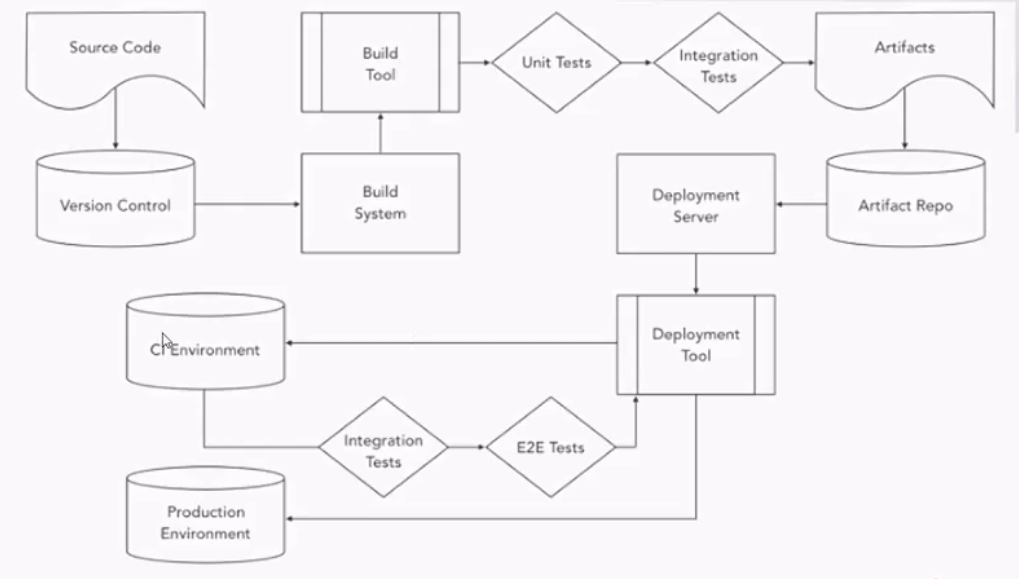
\includegraphics[width=16cm]{bpl}
		\end{center}
	\subsection{CI Flow diagram}
		\begin{center}
			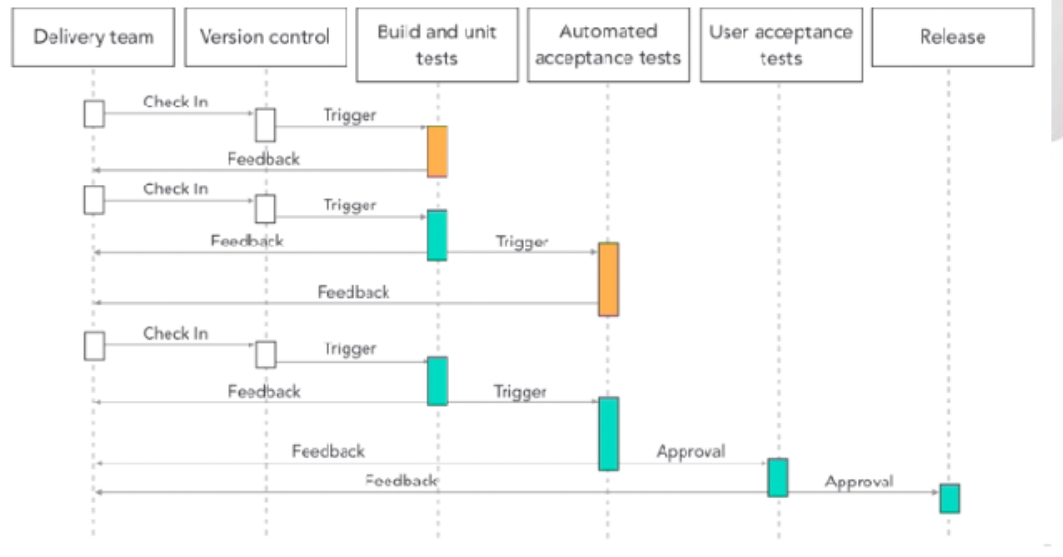
\includegraphics[width=16cm]{fd}
		\end{center}
	\twocolumn
	\subsection{Version control}
		\subsubsection{practices}
			\begin{compactitem}
				\item always use version control 
				\item needs to be used by all teams who touch the code 
				\item build and deploy with a single command 
				\item commit often
				\begin{compactitem}
					\item uncompleted features hidden behind a feature flag 
				\end{compactitem}
				\item easy to understand commit messages 
				\item don’t commit broken code 
				\item commit hooks enforce quality 
					\begin{compactitem}
						\item pre-commit hook => fast local test 
					\end{compactitem}
				\item careful with secrets
			\end{compactitem}
		\subsubsection{Branching}
			\begin{compactitem}
				\item consider a master branch approach
				\item developing off a master gives better performance
				\begin{compactitem}
					\item no need for a lot of branching and pull requests 
					\item mechanism to handle changes should be small and easy to understand
				\end{compactitem}
			\end{compactitem}
		
		\subsection{CI principles and practices}
		\begin{compactitem}
			\item VC server => CI server
			\item CI is practise
			\item Open source tool jenkins
			\item CI as service
			\item Start with a clean environment 
			\begin{compactitem}
				\item  Don’t maintain the previous run 
			\end{compactitem}
			\item Pass the coffee test 
			\begin{compactitem}
				\item  Code commit to receiving results less than 5 minutes
			\end{compactitem}
		\end{compactitem}
			\subsubsection{CI culture} 
				\begin{compactitem}
					\item  Run tests locally before committing
					\item Do code reviews 
					\item Don’t commit new code to broken builds 
					\item Don’t leave the build broken No “coat commits”
					\item Don’t remove failing tests
				\end{compactitem}
		\subsection{Review}
			\begin{center}
				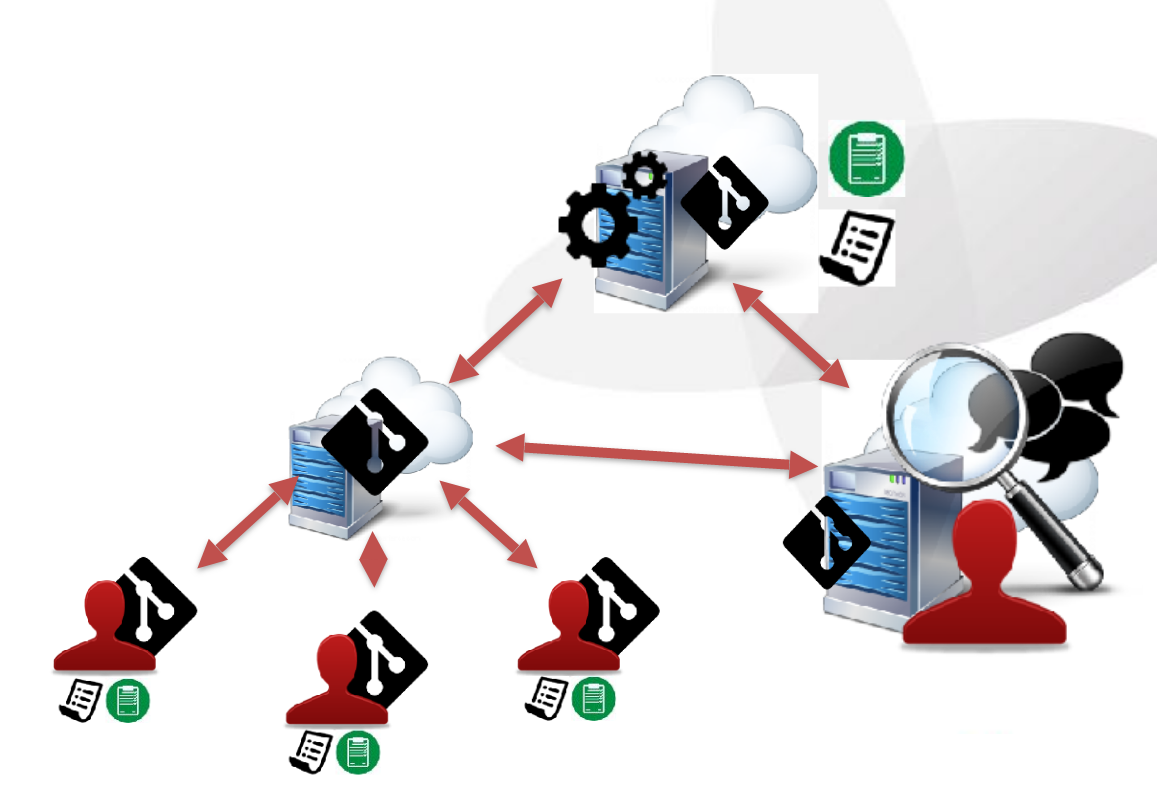
\includegraphics[width=9cm]{rev}
			\end{center}
			Review visszajelzés
			\begin{compactitem}
				\item 0: nem tudom eldönteni
				\item -1: szerintem ne
				\item -2: semmiképp ne
				\item 1: szerintem igen
				\item 2: jó, mehet	
			\end{compactitem}
		\newpage
		\subsection{Notifications on build progress}
			\begin{compactitem}
				\item Commit 
				\item Build start 
				\item Build complete 
				\item Deploy to stage 
				\item Deploy to production 
				\item Undeployed code for more than an hour
				\item Event in the monitoring tool 
				\begin{compactitem}
					\item Collerating errors to code changes
				\end{compactitem}
			\end{compactitem}
		\subsection{Artifacts}
			Kész lefordítótt kódok amik kiszállításra fog kerülni teszt után
			\subsubsection{Reliability}
				what you tested goes into production
			\subsubsection{Composability}
				\begin{compactitem}
					\item language version 
					\item library version 
					\item specific compiler or interpreter 
					\item other dependencies 
				\end{compactitem}
			\subsubsection{Security}
				control over what goes into the package
			\subsubsection{Shareability}
				well understood construct for consuming your code
		\newpage
		\subsection{Plan ahead}
			Artifact megtervezése
			\subsubsection{Packaging formats}
			\begin{compactitem}
				\item RPM 
				\item debian package 
				\item Python package repo 
			\end{compactitem}
			\subsubsection{Dependency management}
				dependency definition in packaging
			\subsubsection{Artifact repositories }
				\begin{compactitem}
					\item Nexus 
					\item JFrog Artifactory 
					\item Apache Archiva 
					\item etc
				\end{compactitem}
		\newpage
		\subsection{Testing, Types of testing}
			Good tests are: fast, reliable, isolate failures
			\subsubsection{Unit testing}
				\begin{compactitem}
					\item Performed at build time on a single unit of code and/or artifact without the use of external dependencies or deployment
					\item JUnit, XUnit, Rspec, etc
				\end{compactitem}
			\subsubsection{Integration testing}
				\begin{compactitem}
					\item Bringing together pieces of your application as it needs to use external dependencies 
					\item full app, API, running server 
					\item RAML, serverspec
				\end{compactitem}
			\subsubsection{End-to-end (E2E) testing}
				\begin{compactitem}
					\item exercise the full flow of an application 
					\item Selenium, protractor
				\end{compactitem}
			\subsubsection{Security testing}
				\begin{compactitem}
					\item looks for flaws in code and runtime to prevent compromises and leaking of data in production 
					\item FindBugs, Fortify, GauntIt
				\end{compactitem}
			\subsubsection{Performance tests}
				\begin{compactitem}
					\item soak tests (napokig futtatjuk, eláztatjuk)
					\item spike tests (stressz teszt magas terhelés)
					\item step tests (lépésenként végrehajtani)
				\end{compactitem}
			\subsubsection{System tests }
			\subsubsection{Acceptance tests }
			\subsubsection{Validation tests}

		\subsection{Terminology}
			\subsubsection{Shift left}
				move testing as early as possible in the dev process
			\subsubsection{Test fixtures}
				set of objects used to run a test in a well known environment
				\begin{compactitem}
					\item dataset, server with known configuration, etc 
					\item artifacts and should be built and managed like one
				\end{compactitem}	
			\subsubsection{System under test (SUT)}
				the application and system on which you are running the tests
			\subsubsection{Cycle time}
				time from work starting on item to delivery into production
			\subsubsection{Lead time }
				time from requesting an item until it’s delivered into production
			\subsubsection{Mocking or stubing }
				code to stand in for external dependencies to enable unit tests
		\newpage
		\subsection{Testing philosophy}
			\subsubsection{Test driven development (TDD) }
				\begin{compactitem}
					\item writing a failing test first, and then writing the code to pass 
					\item refactoring to make it cleaner 
				\end{compactitem}
			\subsubsection{Behavior driven development (BDD)}
				writing tests in a simple end user behaviour centric language 
			\subsubsection{Acceptance test driven development (ATDD)}
				agreeing on acceptance tests before development to estabilish what to deliver
		\subsection{TDD}
			Never just hope that your code works
			Prove it, Again...,... and again... , ... and again... , From the first line of code... ,... to deployment.
			The easiest way is automated testing.
			\begin{compactitem}
				\item Write a test 
				\item Watch the test fail 
				\item Write application logic - as simple as possible 
				\item Pass the test 
				\item Refactor, removing duplication 
				\item Pass the test again
			\end{compactitem}
		\subsection{Does unit testing replace all other testing?}
			There are plenty of other necessary tests 
			beta testing, performance testing, stress testing, integration testing, usability testing ,etc. So, the answer is definitely NOT!
		\subsection{Does TDD work for everything?}
			There is much more: Multi-threading, Security testing, UI testing, Game development, etc.
		\subsection{Unit testing frameworks}
			For creating, running and managing automated unit tests
			XUnit, SUnit - Smalltalk, JUnit - Java, NUnit - .NET, PyUnit - Python, CppUnit - C++, OCUnit - Objective-C
		\subsection{Assertion}
		Sanity check. Positive: These two strings are equal, This integer is positive. Negative :This object in not NULL. Not the generic flow of code: exceptions, error handling, diagnostic dialog boxes. FAIL NOW!
		\subsection{Can I change the order of tests?}
			\begin{compactitem}
				\item  The order shouldn’t matter 
				\item Controlling suggests dependencies - avoid at all costs 
				\item Unit tests are not to test the whole application 
				\item Unit tests are are only for testing individual units 
				\subitem In isolation
			\end{compactitem}
		\newpage
		\subsection{Why mocking?}
			\begin{compactitem}
				\item Why mocking?
				\item Real object hasn’t been written yet 
				\item UI needs human interaction 
				\item Slow or difficult to set up 
				\item External resource (file system, database, network, printer, etc.) 
				\item Non-deterministic behavior
			\end{compactitem}
		\subsection{Mock Object Frameworks}
			Provide structure for defining mock objects, May remove the need to create a custom class
			Can help in generating method stubs, 
			Often provide prearranged mock objects.
			\begin{compactitem}
				\item File stream 
				\item Console 
				\item Network 
				\item Printer 
				\item etc.
			\end{compactitem}
		\onecolumn
		\subsection{Measuring code coverage}
			\begin{center}
				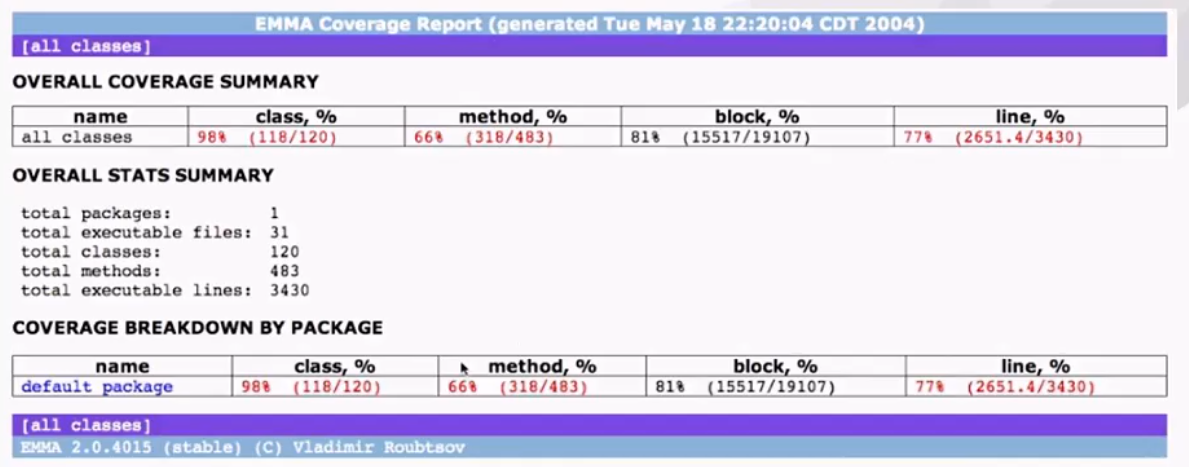
\includegraphics[width=18cm]{cc}
			\end{center}
		\subsection{What to test?}
			Test every branch, if, else, and, or, case, for, while, polymorphism. “Test until fear turns to boredom”. Use code coverage tools.
		\subsection{What to avoid}
			\begin{compactitem}
				\item Interaction with a database or file system 
				\item Require non-trivial network communication 
				\item Require environment changes to run 
				\item Call complex collaborator objects 
				\item Unit tests != other tests 
			\end{compactitem}
		
		\subsection{Testing metrics}
			\subsubsection{Cycle time}
				time from the start of work to delivery 
			\subsubsection{Velocity}
				Value delivered per unit time 
			\subsubsection{Customer satisfaction }
				How well a product/service met the customer’s needs	
				\begin{compactitem}
					\item NPS (Net Promoter Score) 
					\item Bug reports
				\end{compactitem}
			\twocolumn
		\subsection{70-20-10\%}
			\begin{center}
				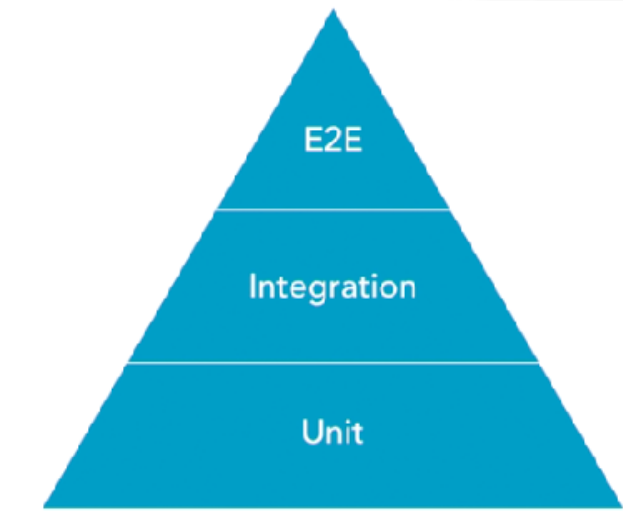
\includegraphics[width=8cm]{pi}
			\end{center}
		\subsection{Deployment}
			\begin{compactitem}
				\item Same artifact 
				\item Same way 
				\item Same (or at least similar) environment 
				\item Same smoke tests at the end of every deployment 
				\item Small batches 
				\item Changes loosely coupled as much as possible 
				\item Separate deploy and release
				\begin{compactitem}
					\item Blue/green deployment (Zöld élő, kékre új deploy, ezt nem használják az ügyfelek, ha minden teszt sikeres a kékből lesz az új zöld)
					\item Feature flags to toggle parts of the code
				\end{compactitem}
			\end{compactitem}
		\subsection{Best practices}
		\begin{compactitem}
			\item Each developer is responsible for their check-in 
			\item Small changes 
			\item Build quality in 
			\item Don’t check in broken builds 
			\item Automate high quality testing 
			\item Run tests before check in 
			\item Fix inconsistent tests 
			\item Don’t ignore or disable tests 
			\item Automate deployment 
			\item Keep the build and deployment fast
		\end{compactitem}
		\onecolumn
		\subsection{A real life example}
			\begin{center}
				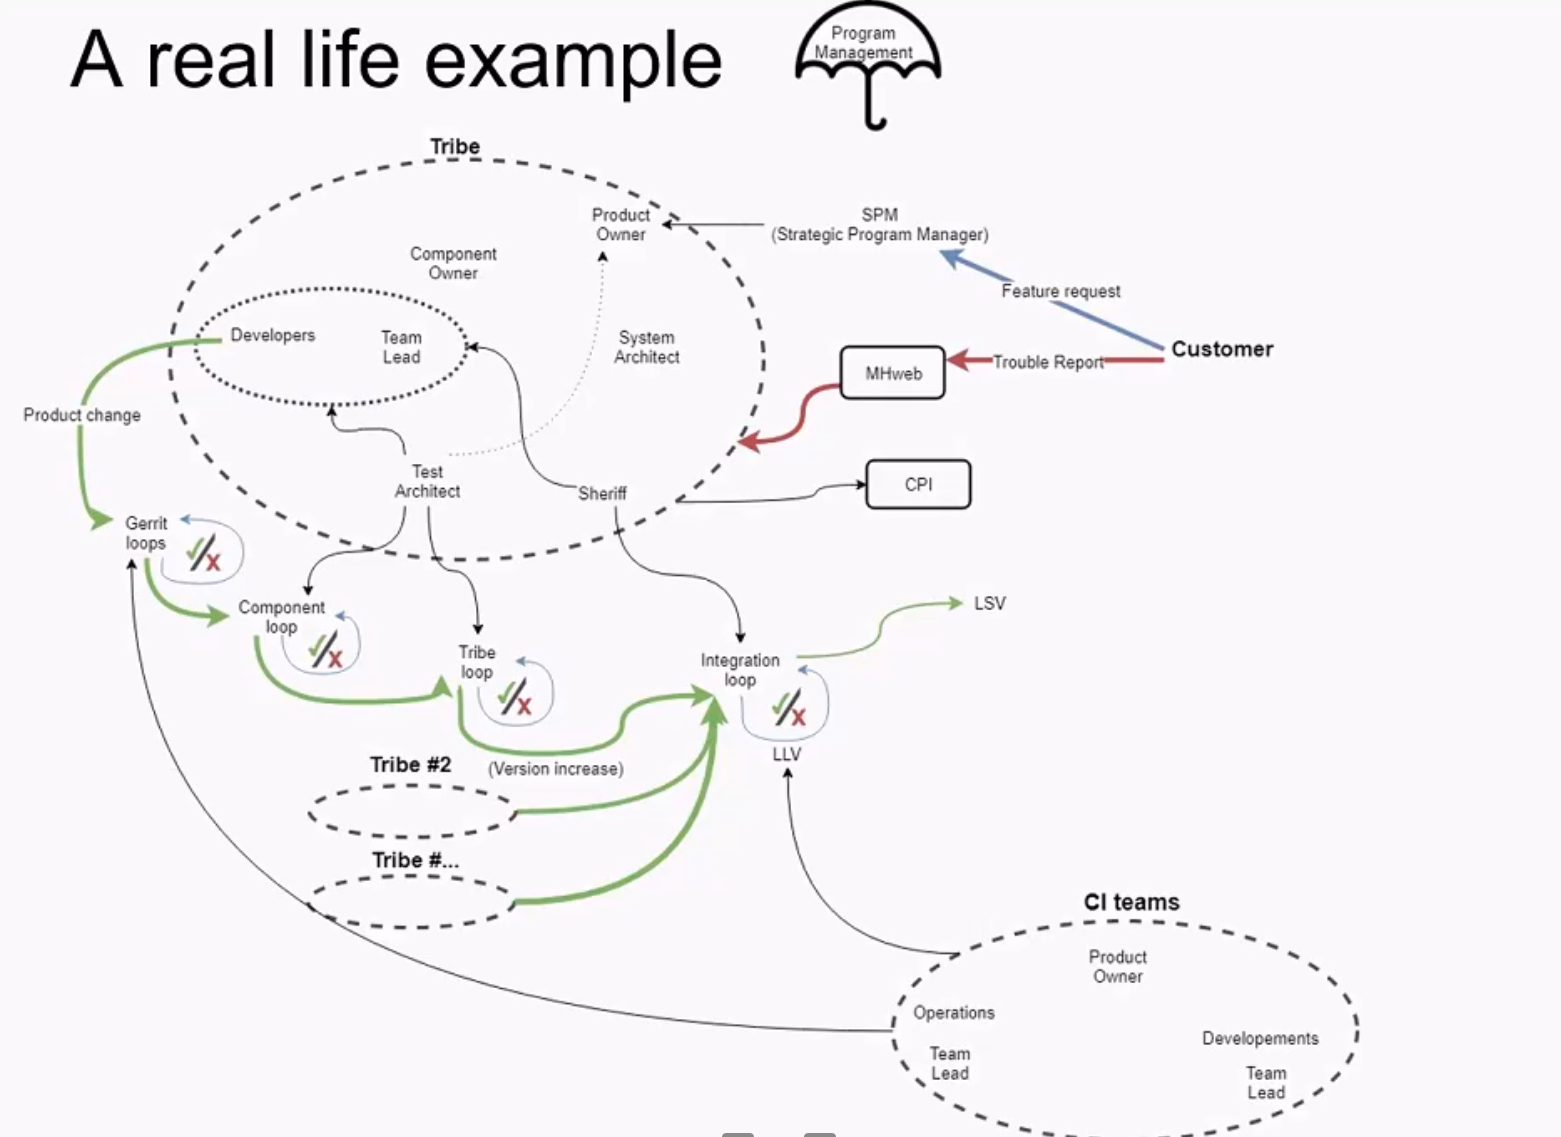
\includegraphics[width=20cm]{ex1}
			\end{center}
		\subsection{The full picture}
			\begin{center}
				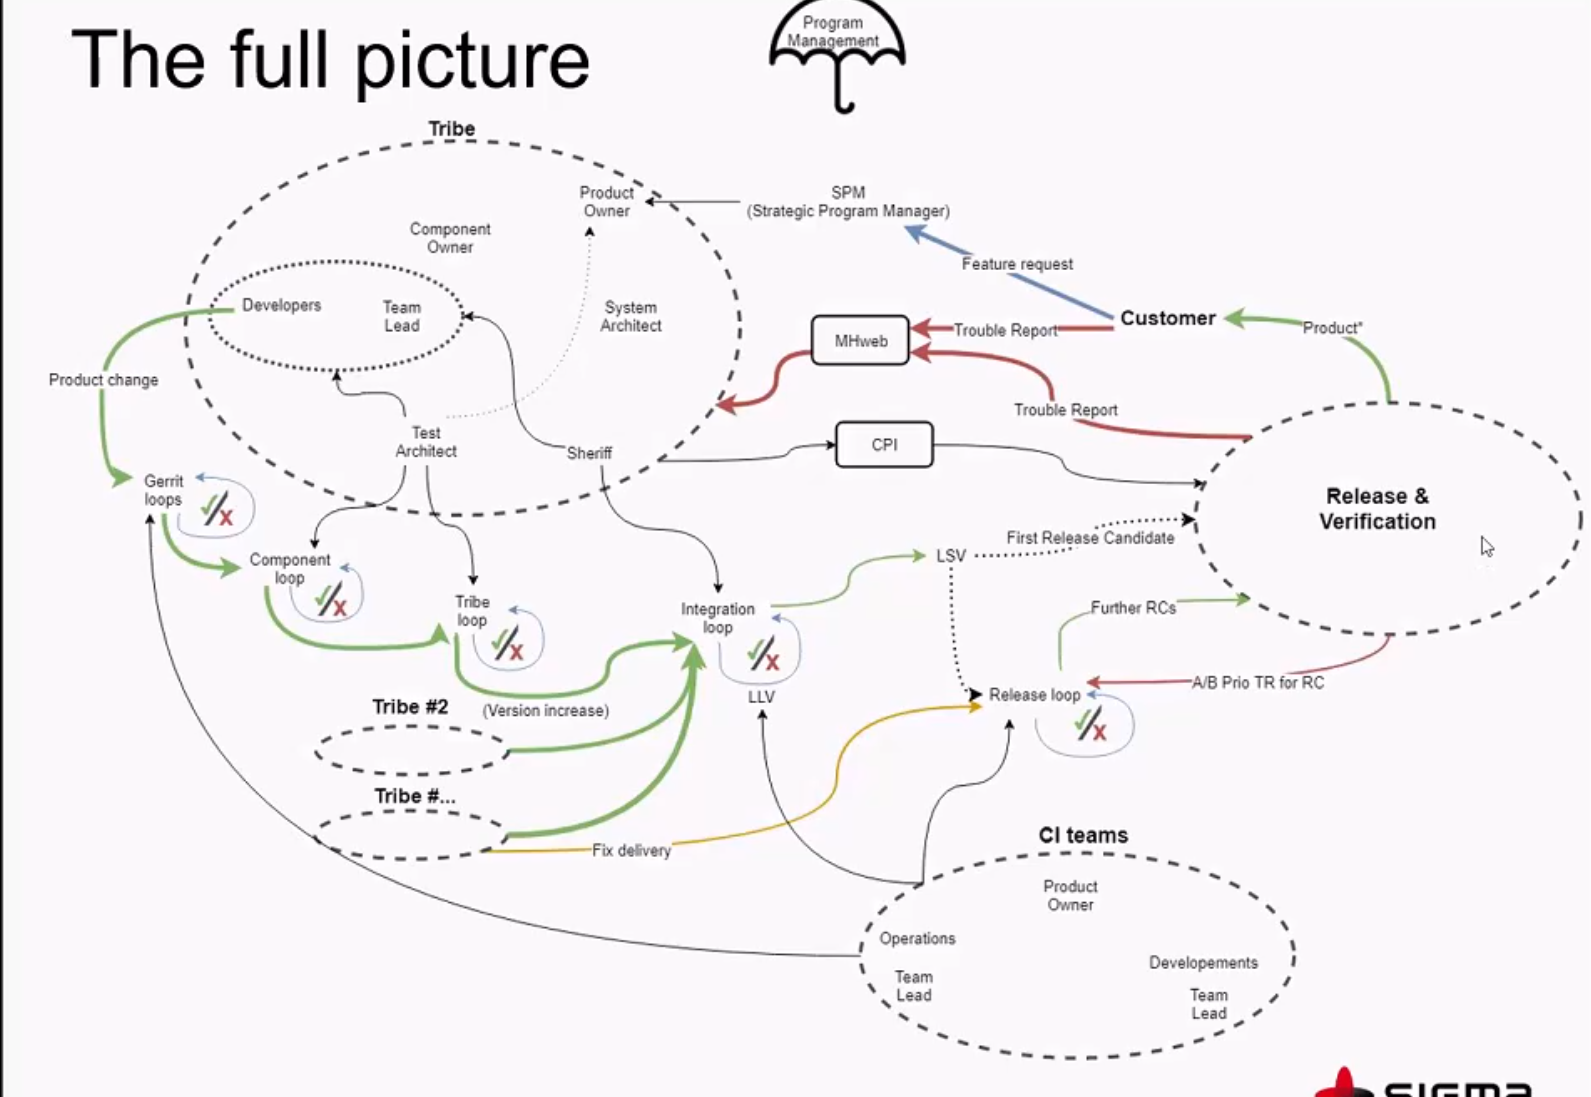
\includegraphics[width=19cm]{fp}
			\end{center}
		
	\section{Selenium}
		

\end{document}